%%%%%%%%%%%%%%%%%%%%%%%%%%%%%%%%%%%%%%%%%%%%%%%%%%%%%%%%%%%%%%%%%%%%%%
%%                     Not
%%%%%%%%%%%%%%%%%%%%%%%%%%%%%%%%%%%%%%%%%%%%%%%%%%%%%%%%%%%%%%%%%%%%%%
%\color{blue}
\subsection{Glyph: \glyph{Not}}\label{sec:not}

The glyph \glyph{not} is used to denote that the \glyph{interactor} linked as input .....

\question{NLN}{I am not sure what it means actually} 

\begin{glyphDescription}
 \glyphSboTerm SBO:0000238 ! not.
 \glyphOrigin One interactor (section~\ref{sec:interactors}) or logical operator (section~\ref{sec:logic}).
 \glyphTarget  One modulation (section~\ref{sec:modulation}), stimulation (section~\ref{sec:stimulation}), inhibition (section~\ref{sec:inhibition}), necessary  stimulation (section~\ref{sec:necessaryStimulation}), or absolute inhibition (section~\ref{sec:absoluteInhibition}) arc.
 \glyphNode \glyph{Not} is represented by a circle carrying the word ``NOT''.
 \end{glyphDescription}

\begin{figure}[H]
  \centering
  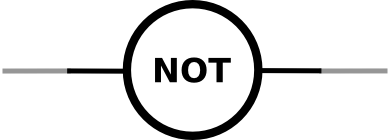
\includegraphics[scale = 0.5]{images/not}
  \caption{The \PD glyph for \glyph{not}.}
  \label{fig:not}
\end{figure}

